\documentclass[a4paper]{article}

\usepackage[utf8]{inputenc}
\usepackage[portuges]{babel}
\usepackage{graphicx}
\usepackage{a4wide}
\usepackage[pdftex]{hyperref}
\usepackage{float}
\usepackage{graphicx}
\usepackage{indentfirst}
\usepackage[small]{caption}


\begin{document}

\title{Projeto Facultativo de Desenvolvimento de Sistemas de Software}
\author{Catarina Machado (a81047)}
\date{\today}

\begin{titlepage}

  %título
  \thispagestyle{empty}
  \begin{center}
  \begin{minipage}{0.75\linewidth}
      \centering
  %engenharia logo
      \includegraphics[width=0.4\textwidth]{imgs/eng.jpeg}\par\vspace{1cm}
      \vspace{1.5cm}
  %titulos
      \href{https://www.uminho.pt/PT}{\scshape\LARGE Universidade do Minho} \par
      \vspace{1cm}
      \href{https://www.di.uminho.pt/}{\scshape\Large Departamento de Informática} \par
      \vspace{1.5cm}

  \maketitle

  \end{minipage}
  \end{center}
  \clearpage

 \end{titlepage}


\begin{abstract}
O presente relatório descreve de forma sucinta o projeto facultativo realizado no âmbito da UC de Desenvolvimento de Sistemas de Software, no terceiro ano do Mestrado Integrado em Engenharia Informática, na Universidade do Minho.
O objetivo do projeto foi desenvolver um sistema capaz de gerir as quotas dos sócios do centro de estudantes do curso (CeSIUM).
\end{abstract}
\pagebreak

\tableofcontents


\pagebreak

\section{Introdução}
\label{sec:intro}

O relatório descreve a forma como os dados foram organizados, as classes que foram utilizadas e inclui também um manual de utilização para a aplicação.

Para a realização deste projeto segui o modelo MVC (Model-view-controller). O trabalho foi realizado utilizando o IntelliJ IDEA.


O objetivo da aplicação é que seja possível visualizar uma lista com todos os sócios do centro de estudantes bem como visualizar os detalhes de um determinado sócio (dados pessoais e quotas pagas). Também será possível adicionar novos sócios ao sistema e registar o pagamento de novas quotas por parte dos sócios.

Na Secção~\ref{sec:estruturadedados} encontram-se as classes que fazem parte do "Model", na secção~\ref{sec:view} estão enumeradas as classes que constituem a "View" do programa e na secção~\ref{sec:controller} encontra-se uma breve descrição da classe que constitui o "Controller". Na secção~\ref{sec:metodos} são apresentados os metódos essenciais para o funcionamento do programa e na secção~\ref{sec:manual} está um manual de utilizador para a plataforma.

\section{Organização dos Dados- Model}
\label{sec:estruturadedados}

Para desenvolvermos este trabalho adotamos as seguintes classes:

\subsection{Classe Sócio}
\label{sec:classesocio}

\begin{verbatim}
    private int numero;
    private String nome;
    private String curso;
    private int ano;
    private String morada;
    private List<Quota> quotas;
\end{verbatim}

\vspace{0.2cm}

Esta classe armazena toda a informação necessária relativa a um sócio, nomeadamente o seu \textbf{número} de sócio, \textbf{nome}, \textbf{curso}, \textbf{ano}, \textbf{morada} e uma \textbf{lista com todas as quotas} já pagas por ele.

\subsection{Classe Quota}
\label{sec:classequota}

\begin{verbatim}
    private double valor;
    private LocalDate data;
\end{verbatim}

\vspace{0.2cm}

A classe Quota armazena a informação relativa ao pagamento de uma quota, nomeadamente o \textbf{valor} e a \textbf{data} em que foi realizada.

\subsection{Classe GestaoSocios}
\label{sec:classegestaosocios}

\begin{verbatim}
    private Map<Integer, Socio> socios;
\end{verbatim}

\vspace{0.2cm}

Esta classe é a classe "principal" do sistema uma vez que guarda a \textbf{informação de todos os sócios}. Esta informação é guardada num map, onde a chave é o número de sócio.

\subsection{Classe SocioNullException}
\label{sec:classesocionull}

Classe de exceção- quando o sócio a que tentamos aceder não existe (null).


\section{Interface Gráfica}
\label{sec:view}

Para a camada de apresentação do sistema, foram necessárias 6 classes:

\begin{itemize}
\begin{item} \textit{InitialView} -  painel inicial da aplicação, com os botões para cada uma das funcionalidades principais do sistema.\end{item}
\begin{item} \textit{VisualizarSociosView} - encarregue de mostrar uma tabela com todos os sócios.\end{item}
\begin{item} \textit{SocioDetailsView} - apresenta os detalhes relativos a um determinado sócio.\end{item}
\begin{item} \textit{QuotasPagasView} - responsável por mostrar ao utilizador uma tabela com todas as quotas pagas por ele.\end{item}
\begin{item} \textit{NovoSocioView} - formulário para a criação de um novo sócio.\end{item}
\begin{item} \textit{PagarQuotaView} - responsável por mostrar um formulário que permite que um sócio pague uma quota de um determinado valor.\end{item}
\end{itemize}


\section{Controller}
\label{sec:controller}

A classe "GestaoSociosController", está responsável por coordenar a troca de informação entre a interface gráfica e a camada lógica da aplicação, por exemplo, preenche as tabelas da camada de apresentação com os dados da camada lógica, "pega" nos dados introduzidos pelo utilizador aquando da criação de um novo sócio e chama os metódos necessários para que essa informação seja devidamente inserida no sistema, entre outros.

Esta classe também alimenta a aplicação com três sócios, meramente ilustrativos.

\section{Métodos Essenciais}
\label{sec:metodos}

Para a concretização do problema foram criados alguns métodos com o intuito de responder às diferentes necessidades do sistema:

\begin{enumerate}
    \item Visualizar sócios (Figura~\ref{img:visualizarSocios})- método \textbf{getSocios}, da classe GestaoSocios.
    \item Visualizar detalhes de um sócio (Figura~\ref{img:detalheSocio})- método \textbf{getSocio}, da classe GestaoSocios.
    \item Alterar informações de um sócio (Figura~\ref{img:detalheSocio})- método \textbf{alterarInfoSocio}, da classe GestaoSocios.
    \item Visualizar as quotas pagas por um determinado sócio (Figura~\ref{img:detalheSocio})- método \textbf{getQuotas}, da classe Sócio.
    \item Adicionar um novo sócio (Figura~\ref{img:novoSocio})- método \textbf{addSocio}, da classe GestaoSocios.
    \item Pagamento de uma nova quota (Figura~\ref{img:pagarQuota})- método \textbf{pagarQuota}, da classe GestaoSocios, que utiliza o método addQuota da classe Sócio.
\end{enumerate}


\section{Manual de Utilização}
\label{sec:manual}

Quando a aplicação é aberta, o menu que é apresentado é o seguinte:

\begin{figure}[H]
\centering
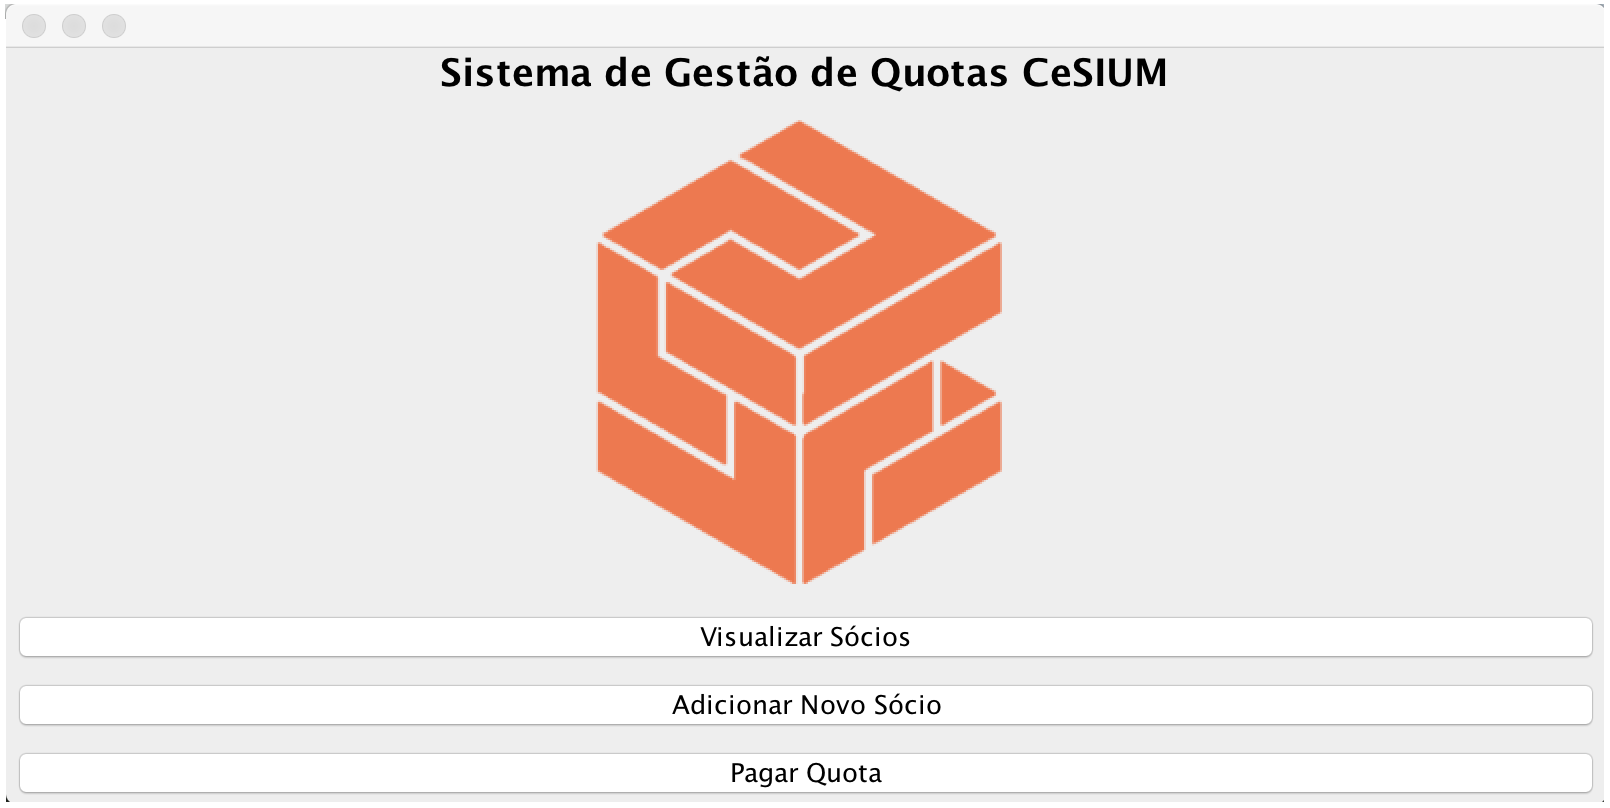
\includegraphics[scale=0.35]{imgs/initialMenu.png}
\caption{Menu inicial da aplicação.}
\label{img:initialMenu}
\end{figure}

Carregando no botão "Visualizar sócios", é apresentada uma tabela com as informações de todos os sócios, tal como se pode ver em seguida:

\begin{figure}[H]
\centering
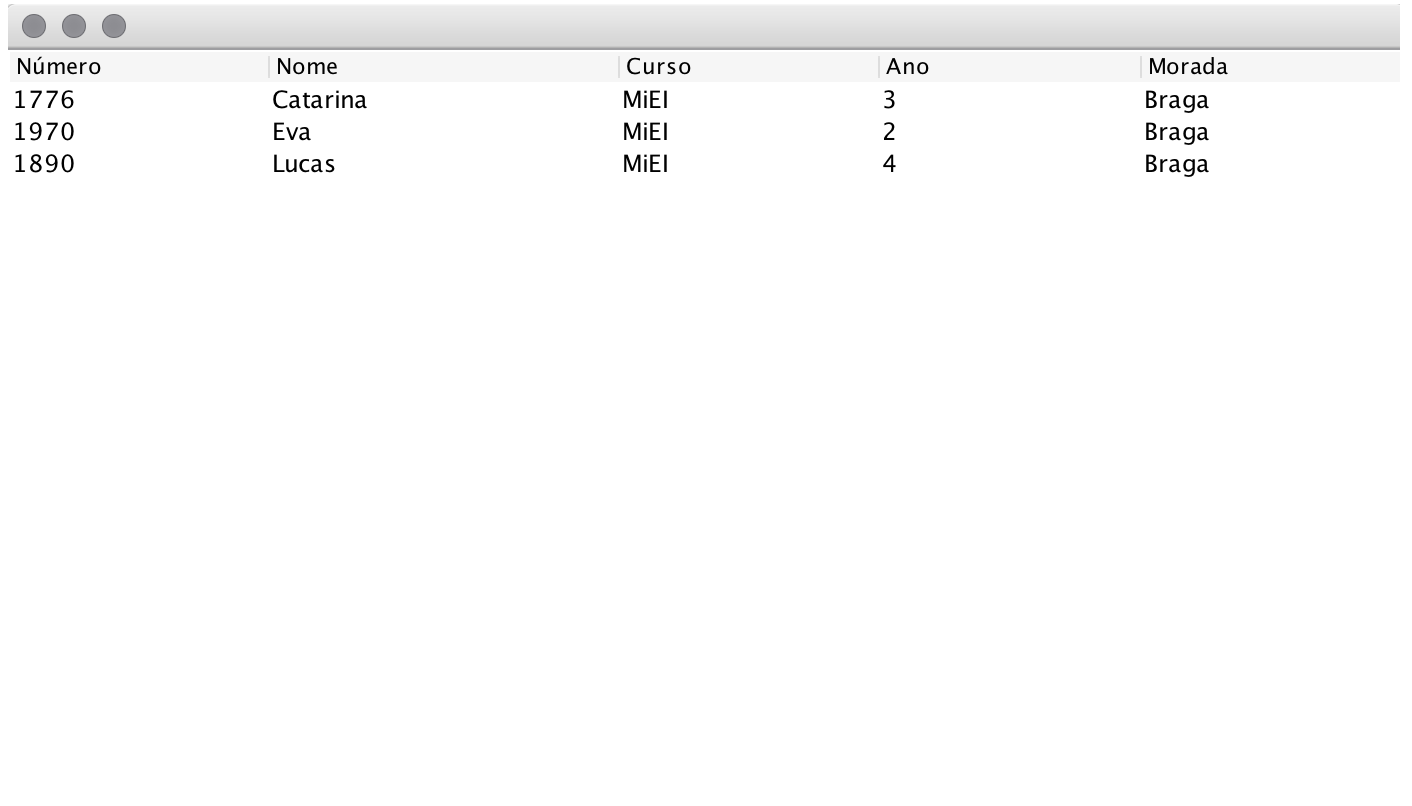
\includegraphics[scale=0.35]{imgs/visualizarSocios.png}
\caption{Visualizar todos os sócios do CeSIUM.}
\label{img:visualizarSocios}
\end{figure}

Carregando num dos sócios apresentado, é aberto um novo menu. Por exemplo, carregando no sócio "Catarina" é aberto o seguinte painel:

\begin{figure}[H]
\centering
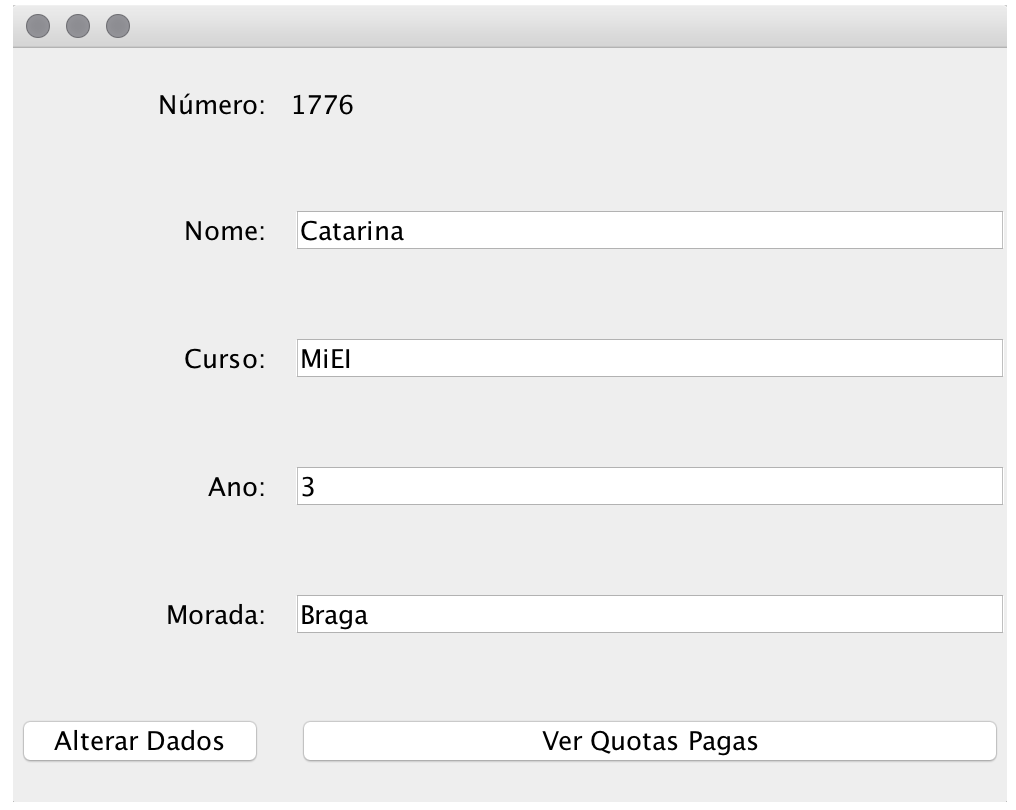
\includegraphics[scale=0.35]{imgs/detalheSocio.png}
\caption{Detalhes de um sócio.}
\label{img:detalheSocio}
\end{figure}

Aqui, o utilizador pode alterar as informações deste sócio. Tem também a possibilidade de ver as quotas pagas por este sócio. Carregando então no botão "Ver Quotas Pagas" aparece o seguinte menu:

\begin{figure}[H]
\centering
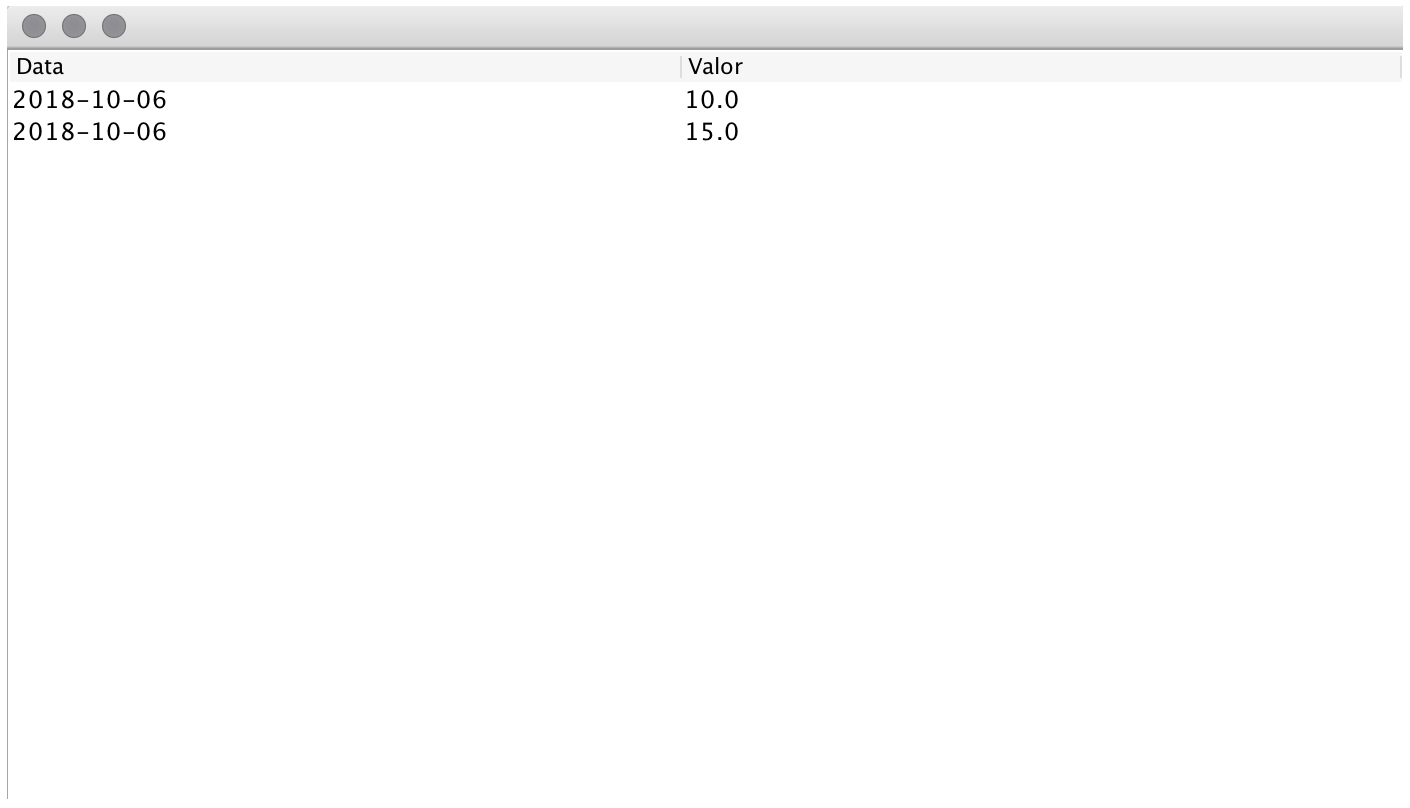
\includegraphics[scale=0.35]{imgs/verQuotas.png}
\caption{Visualizar quotas pagas por um determinado sócio.}
\label{img:verQuotas}
\end{figure}

Olhando novamente para a Figura~\ref{img:initialMenu}, e escolhendo agora o botão "Adicionar Novo Sócio", é apresentado ao utilizador o formulário em seguida:

\begin{figure}[H]
\centering
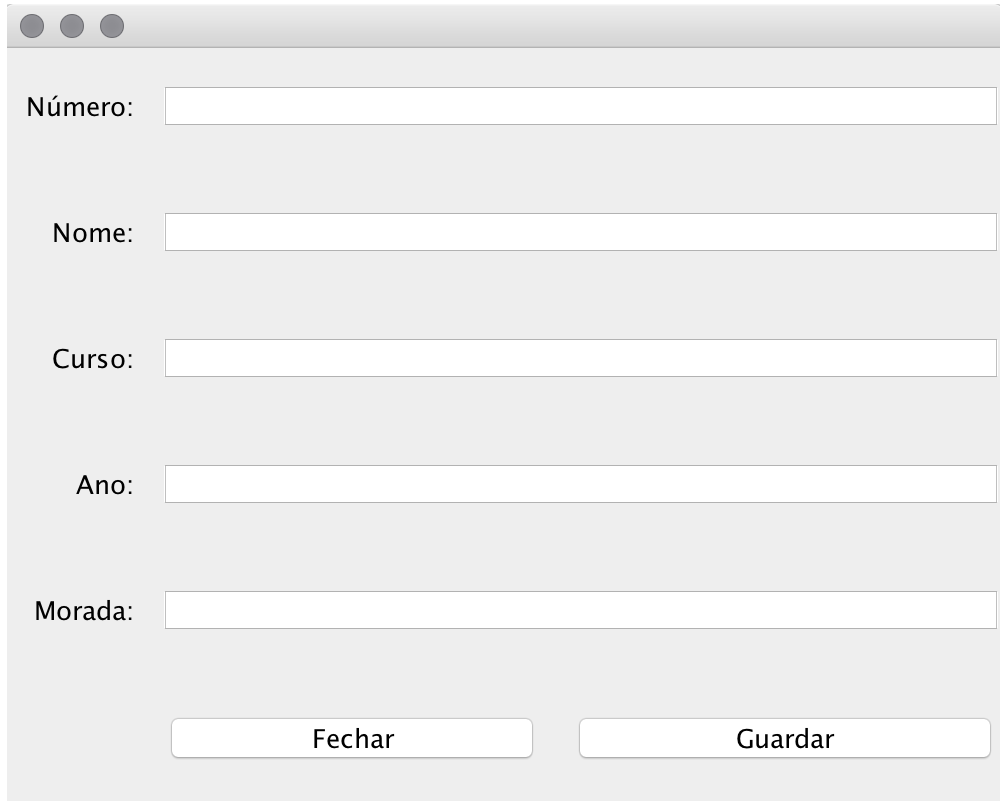
\includegraphics[scale=0.35]{imgs/novoSocio.png}
\caption{Adicionar um novo sócio.}
\label{img:novoSocio}
\end{figure}


Por último, pressionando o último botão do menu inicial (Figura~\ref{img:initialMenu}) o utilizador tem ainda a possibilidade de registar o pagamento de uma nova quota. Este é o painel apresentado caso esta opção seja selecionada:

\begin{figure}[H]
\centering
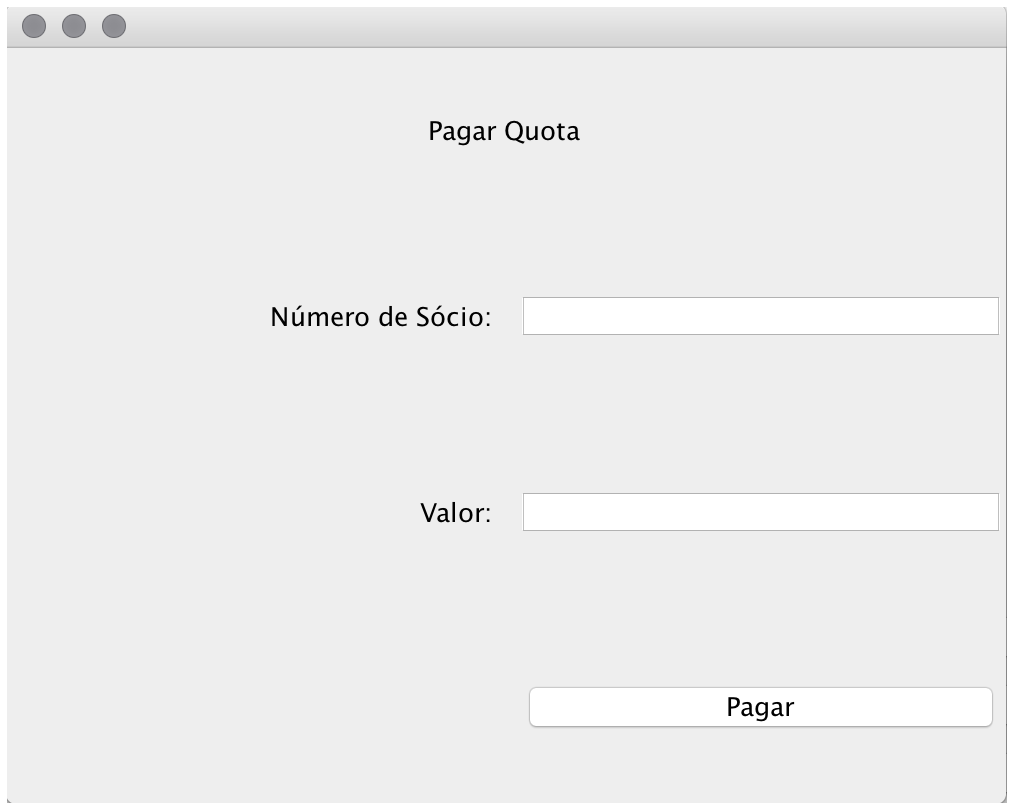
\includegraphics[scale=0.35]{imgs/pagarQuota.png}
\caption{Pagamento de uma nova quota.}
\label{img:pagarQuota}
\end{figure}


Para além destes menus, é também de salientar que existe feedback por parte da aplicação quando existe input por parte do utilizador, fazendo assim com que a UX seja melhorada.

Por exemplo, caso seja adicionado com sucesso um novo sócio ao sistema aparece a seguinte mensagem no ecrã:

\begin{figure}[H]
\centering
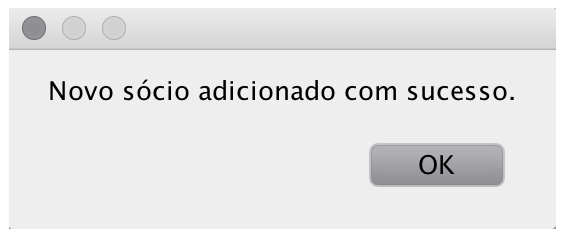
\includegraphics[scale=0.35]{imgs/feedbackNovoSocio.png}
\caption{Feedback positivo novo sócio.}
\label{img:feedbackNovoSocio}
\end{figure}

Caso haja insucesso nesta operação, por exemplo, se não foram inseridos apenas caracteres númericos no ano e no número de sócio aparece a seguinte janela.

\begin{figure}[H]
\centering
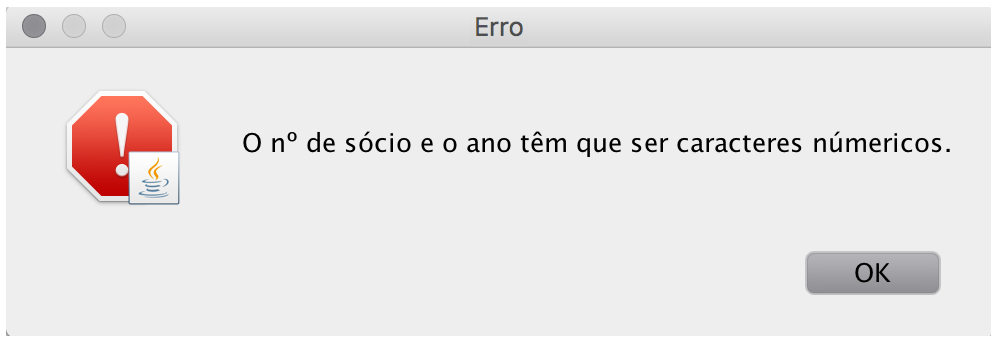
\includegraphics[scale=0.35]{imgs/feedbackNegatNovoS.png}
\caption{Feedback negativo novo sócio.}
\label{img:feedbackNegatNovoS}
\end{figure}

Caso uma nova quota seja efetuada com sucesso, ou seja, o valor inserido seja um caracter númerico e o número de sócio seja um número que já existe é apresentada a seguinte mensagem:


\begin{figure}[H]
\centering
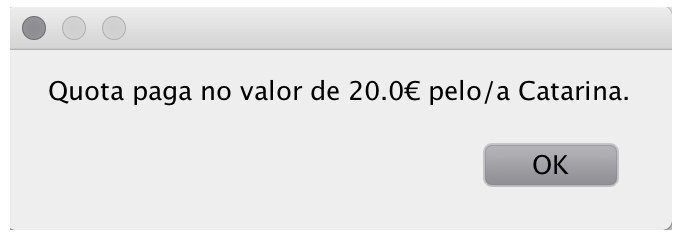
\includegraphics[scale=0.35]{imgs/feedbackQuota.png}
\caption{Feedback pagamento de uma quota.}
\label{img:feedbackQuota}
\end{figure}

Caso, por exemplo, o número de sócio inserido não corresponda a nenhum sócio no sistema é apresentada a seguinte janela:

\begin{figure}[H]
\centering
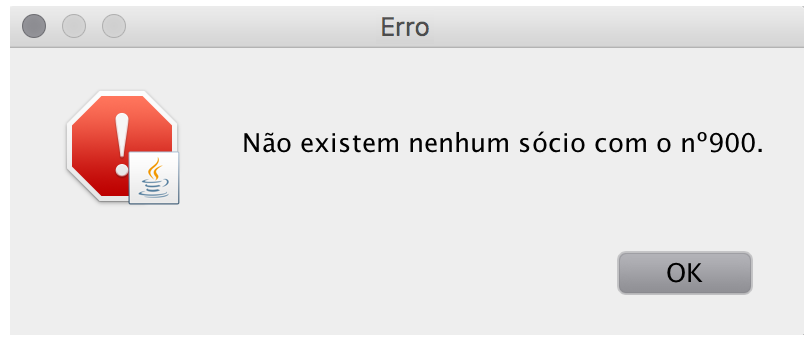
\includegraphics[scale=0.35]{imgs/feedbackNegaNovaQ.png}
\caption{Feedback negativo nova quota.}
\label{img:feedbackNegaNovaQ}
\end{figure}


Quando os dados de um sócio são alterados, aparece a seguinte mensagem:

\begin{figure}[H]
\centering
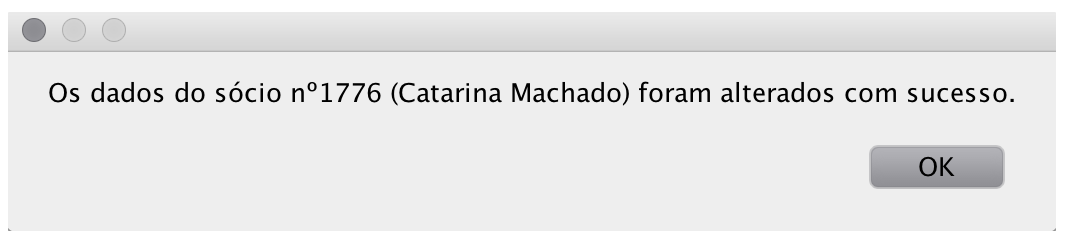
\includegraphics[scale=0.35]{imgs/feedbackAlterarDados.png}
\caption{Feedback Alterar Dados.}
\label{img:feedbackAlterarDados}
\end{figure}

Esses são apenas alguns exemplos de feedback que a aplicação fornece.

\section{Conclusões}
\label{sec:conclusao}

A realização deste mini projeto foi bastante positiva nesta altura do semestre uma vez que me deu a oportunidade de relembrar alguns conceitos de Java e de praticar um pouco mais esta linguagem de programação. Ajudou ainda a praticar o padrão de arquitetura de software MVC.

Gostei do resultado final da aplicação no que diz respeito à UI e também à forma como as classes se encontram implementadas. No entanto, gostava de ter povoado a aplicação com mais funcionalidades, por exemplo, haver um menu com uma tabela com a informação de todas as quotas pagas por todos os sócios, haver uma notificação dos sócios que têm quotas em atraso ou até dar mais informações estatísticas como por exemplo o número total de sócios do centro de estudantes.



\end{document}
